\hypertarget{index_overview}{}\section{Overview}\label{index_overview}

Recent system-on-a-chip designs have integrated CPU, GPU, and other
accelerator devices onto a single chip with a shared high-bandwidth
memory system.  In fact, these single-chip designs are now widely
used in many computing markets including cellphones, tablets,
personal computers, and game consoles. The Heterogeneous System
Architecture (HSA) builds on the close physical integration of
accelerators that is already occurring in the marketplace, and takes
the next step by defining standards for uniting the accelerators
architecturally.  The HSA specifications includes requirements for
virtual memory, memory coherency, architected dispatch mechanisms,
and power-efficient signals.   
HSA refers to these accelerators as “components”.  The system
architecture defines a consistent base for building portable
applications that access the power and performance benefits of the
dedicated hsa components.   Many of these components, including GPUs
and DSPs, are capable and flexible processors that have been
extended with special hardware for accelerating parallel code.
Historically these devices have been difficult to program due to a
need for specialized or proprietary programming languages.  HSA aims
to bring the benefits of these components to mainstream programming
languages using similar or identical syntax to that which is
provided for accessing multi-core CPUs.

In addition to the system architecture, HSA’s “Programmer’s
Reference Guide” defines HSAIL - a portable, low-level, compiler
intermediate language designed for parallel computing.  

\begin{description}
\item[Portable:] The HSAIL language is an open-standard, supported by
multiple vendors in the HSA Foundation, and is portable across
vendors and product generations, so that applications which use
HSAIL are guaranteed to run on future hardware that supports the
HSAIL standard.  
\item[Low-level:] HSAIL’s representation is just above the machine
instruction set.  Most optimizations including register allocation
are intended to be performed by the compiler that generates HSAIL.
HSAIL code is translated to the host instruction set by a tool
called the “finalizer”.  Each component will provide its own
implementation of the finalizer.  The finalization step is intended
to be lightweight, fast, and simple.  Importantly, the finalizer
step does not involve a complex compiler.  Applications which
contain HSAIL should not see different functional or performance
behavior from new finalizer versions that might be deployed in the
field after the application ships.
\item[Designed for parallel computing:] HSAIL is intended to represent
the parallel sections of an application.  It complements but does
not replace the host code – host code still exists and is used for
the serial portion of the application.  HSAIL represents a single
“lane” of execution, and the parallelism is expressed in the grid
dimensions that are specified when the HSAIL kernel is dispatched to
a target component.  In this way, HSAIL does not encode a specific
“vector width” and can be used to represent a variety of different
parallel computing devices.
\end{description}

For more information on HSAIL, refer to the HSA Programmer’s
Reference Guide.  

The final piece of the puzzle is the HSA Core Runtime API.  The core
runtime is a thin, user-mode API that provides the interfaces
necessary for the host to launch compute kernels to the available
components.  This document describes the architecture and APIs for
the HSA Core Runtime.  Key sections of the runtime API include:

\begin{itemize}
\item Error handling
\item Runtime initialization (open/close)
\item Topology and Component Discovery
\item Signals and Synchronization
\item Architected Dispatch
\item Memory Management
\end{itemize}

In summary, there are three specifications provided by the HSA
Foundation:
\begin{description}
\item[HSA System Architecture Requirements:] Architectural foundation for
how HSA components share memory and communicate work requests.
\item[HSA Programmer’s Reference Manual:] Describes HSAIL, a low-level,
portable compiler IR appropriate for use as compiler intermediate
language.
\item[HSA Runtime Specification:] This document.  Describes the host-side
API for controlling the launch of HSAIL kernels.
\end{description}

The remainder of this document describes the HSA software
architecture and execution model, and includes functional
descriptions for all of the HSA APIs and associated data structures. 

\begin{figure}
  \centering
  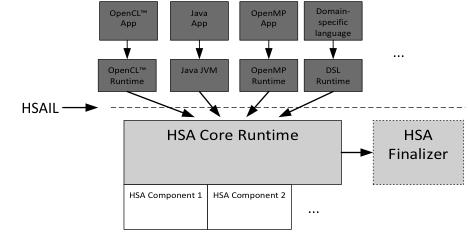
\includegraphics[width=0.5\textwidth]{swarch}
  \centering
  \caption{HSA Software Architecture}
  \label{fig:swarch}
\end{figure}

Figure~\ref{fig:swarch} shows how the HSA Core Runtime fits into a
typical software architecture stack.

At the top of the stack is a programming model such as OpenCL™,
Java, OpenMP, or a domain-specific language (DSL).   The programming
model must include some way to indicate a parallel region that can
be accelerated.  For example, OpenCL has calls to
\texttt{clEnqueueNDRangeKernel} with associated kernels and grid ranges.
Java has the stream and lambda APIs, which provide support for both
multi-core CPUs and HSA Components.  OpenMP contains OMP pragmas
that mark parallel for loops and control other aspects of the
parallel implementation.  Other programming models can also build on
this same infrastructure.

The language compiler is responsible for generating HSAIL code for
the parallel regions.  HSA supports several options for when HSAIL
is generated and finalized.  One possibility is that the HSAIL is
generated by a high-level compiler and then embedded in the
application binary.  In this case, the finalizer is run when the
application loads and will convert the HSAIL to machine code for the
target machine.   Another option is that the HSAIL is finalized when
the applications is built, or the machine cod  The HSA Finalizer is
an optional component of the HSA Core Runtime, which may reduce the
footprint of the HSA software on systems where the finalization is
done before runtime. 

Each language also includes a “language runtime” that connects the
language implementation to the HSA Core Runtime.   When the language
compiler generates code for a parallel region, it will include calls
to the HSA Runtime to set up and dispatch the work to the HSA
Component.   The language runtime is also responsible for
initializing HSA, and may utilize other HSA core runtime features as
well.  

The API for the HSA core runtime is standard across all HSA vendors,
such that languages which use the HSA runtime can run on the
different vendors that support the API.  Each vendor is responsible
for supplying their own implementation which supports the hsa
component(s) in the vendor’s platform.   HSA does not provide a
mechanism to combine runtimes from different vendors; instead
vendors must provide a single runtime which supports all the
components in the platform.
The implementation of the HSA Runtime may include kernel-level
components (typical for hardware components) or may be entirely
user-space (simulators or CPU implementations).     

\hypertarget{glue}{}\section{ Infrastructure and Execution
Flow}\label{glue}

\diffblock{
\hypertarget{executionmodel}{}\section{Execution
Model}\label{executionmodel}
}
\DIFdelbegin \DIFdel{Host/HSAIL – brief intro that describes host running host code
include HSA runtime, components running HSAIL.
}\DIFdelend 

\diffblock{\hypertarget{archdispatch}{}\subsection{Architected Dispatch}
\label{archdispatch}}
Core runtime exposes several details of the HSA hardware,
including architected dispatches and support for execution control.
The overall goal of the core runtime design is to provide a
high-\/performance dispatch mechanism that is portable across
multiple H\-S\-A vendor architectures. Two vendors with the same
host I\-S\-A but different H\-S\-A-\/compliant G\-P\-Us will be able
to run the same unmodified binary, because they support the
H\-S\-A-\/architected A\-Q\-L interface and supply a library
that implements the architected core runtime A\-P\-I. 

In order for user-level applications to use the HSA system and HSA
components, they need to write HSAIL programs and compile and
execute these programs using user mode queues and AQL commands.  The
HSA Programmer’s Reference Manual (PRM) defines HSAIL Virtual ISA
and Programming Model, serves as a Compiler Writer’s Guide, and
defines Object Format (BRIG). The HSA runtime helps setup the
execution via API calls and data structures to support architected
features.

The HSA core runtime realizes architected dispatch. Architected
dispatch is the key feature in an HSA system that enables a
user-\/level application to directly issue commands to the HSA
Component hardware.  Architected dispatch differentiates it from
other higher-\/level runtime systems and programming models\-: other
runtime systems provide software A\-P\-Is for setting arguments and
launching kernels, while H\-S\-A architects these at the hardware
and specification level.  The critical path of the dispatch
mechanism is architected at the H\-S\-A hardware level and can be
done with regular memory operations and runtime provided wrapper
API.  Fundamentally, the user creates user mode queues and an
A\-Q\-L Packet in memory, and then signals the HSA component to
begin executing the packet using light weight operations (which may
be wrapped with A\-P\-I calls).

This section describes various features core runtime provides to
support architected dispatch as steps that a user needs to take to
utilize runtime.

\subsection{Initial Setup}
One of the first steps in the setup is that of device discovery.
Device discovery is performed at the initialization of the core
runtime and information is made available to the user as data
structures. Section~\ref{topology} describes these structures.
The next step in the setup is creation of the
component queues. Queues are an HSA architected mechanism to submit
work to the HSA component HW. The interfaces for queue creation 
are defined in Section~\ref{architected_queue}. Different
components may provide
implementation-\/specific code under the core A\-P\-I for these
functions. H\-S\-A runtime also includes mechanisms to provide
implementation-\/specific data as part of the dispatch, provided
such data can be computed at compile time. 

\subsection{Compilation Flow}
Once an HSAIL program is written or generated by a higher-level
compilation step, it needs to be \emph{assembled} to generate a
BRIG. BRIG is the HSAIL object format and is specified in the PRM. 
HSA runtime defines API call to compile the BRIG and generate a code
object that has sufficient information to execute the user
program. The details of this compilation process and symbol
resolution are discussed in Section~\ref{finalizerchapter}.

\subsection{Execution of Kernel}
The Systems Architecture Requirements (SAR) document specifies the
structure of the \emph{packets} (i.e. commands) that can be placed on
the HSA user mode queues for the component HW to execute them. The
format of the packets is architected and they are referred to as
Architected Queuing Language (AQL) packets. One of the types of AQL
packets is a dispatch AQL packet.
The user can now create an AQL packet
and initialize it with the code object obtained from the
finalization step, including the
allocation of memory to hold the kernel arguments and the
spill/arg/private memory. 
The interface for kernel arguments between the runtime and the
kernel I\-S\-A (instruction set architecture) is also architected at
the H\-S\-A level. This is covered in the H\-S\-A\-I\-L A\-B\-I
(this is discussed in
Section~\ref{coreapi_HSAIL_ABI}),
which specifies the in-\/memory layout of the kernarg segment. Users
can determine the layout of the kernarg memory segment at compile
time merely by examining the signature of the H\-S\-A\-I\-L
function. The finalizer is required to support this A\-B\-I and thus
there is no need for runtime metadata to specify the position or
format of arguments.
This step can be done once for each A\-Q\-L packet creation.

Optimized implementations can cache the
result of this step and re-\/use the A\-Q\-L packet for subsequent
launches. Care must be taken to ensure that the A\-Q\-L Dispatch
packet (and the associated kernel and spill/arg/private memory) is
not re-\/used before the launch completes. For simple cases, (that
is, a single-\/thread, synchronous launch, the
AQL dispatch packet(s) can be declared as a static variable
and initialized at the same time the code is finalized. More
advanced cases can create and track several
AQL Dispatch packet(s) for a single kernel code object.

HSA HW defines a packet process for processing these packets and a doorbell
mechanism to inform the packet processing HW that packets have been
written into the queue. The Core runtime defines a structure and update
API to inform the HW that the dispatch packet has been written to the
queue. Different packet formats and states of a packet are discussed
in Section~\ref{AQL}. Section~\ref{architected_queue} discusses the
queue creation and various states the queue can be in, once it is
created.

Once the packet is written and the HW is informed by way of the
doorbell, the execution can start. The execution happens
asynchronously. The user is free to write more packets for executing
other kernels in the queue. This activity can overlap the actual
execution of the kernel.

\subsection{Determining Kernel Completion}
HSA SAR defines signals as a mechanism for communication between
different parts of a HSA system. Signals are defined as opaque
objects in the HSA core runtime and APIs have been defined to send a
value to the signal and wait for a value at the signal,
Section~\ref{signals} discusses signals in detail. The AQL dispatch
packet has a provision for the user to pass in an opaque signal.
When the HSA Component HW observes a valid signal in the AQL packet,
it sends a value to this signal when execution of the kernel is
complete (success or error). The user can wait on this signal to
determine kernel completion. Errors and their
meaning are discussed in Section~\ref{error}.
\begin{framed}
\lstinputlisting{main.c}
\end{framed}
